\documentclass[]{report}

\usepackage{graphicx}
\usepackage{pdflscape}


% Title Page
\title{Scrum Documentation \\ Movie Database System}
\author{Mathias Pedersen}


\begin{document}
\maketitle

\chapter*{Table of Change}
%table on changes

\hspace{-2cm}\textbf{Version 2}
 \begin{itemize}
\item[\textit{11/12-2013 Mathias}] \hspace{0.5cm}
\textit{Inserted pictures and text concerning the first two, now done, sprints}


\vspace{0.4cm}

\end{itemize}



\chapter*{Sprint Planning}



\section{Available Time}
\label{sec:Available Time}


\section{Product Backlog}
\label{sec:Product Backlog}



\section{Definition of Done}
\label{sec:Definition of Done}
Definition of done for code:
Done means coded to standards, commented, OCL implemented, unit tested and reviewed by the coders and a second party. Changes affecting documentation or models must be updated accordingly. \\


\noindent Definition of done for documentation:
Documentation is to be done in Latex, with all relevant models included. Sections must have a high quality of writing and be reviewed by a peer. \\
Changes must be documented in the table of change with data and pointing to the relevant section.

\newpage
\chapter{Sprint 1}
\label{chap:Spring 1}


\section{Backlog}
Below is the backlog for our first sprint
\begin{figure}[h]
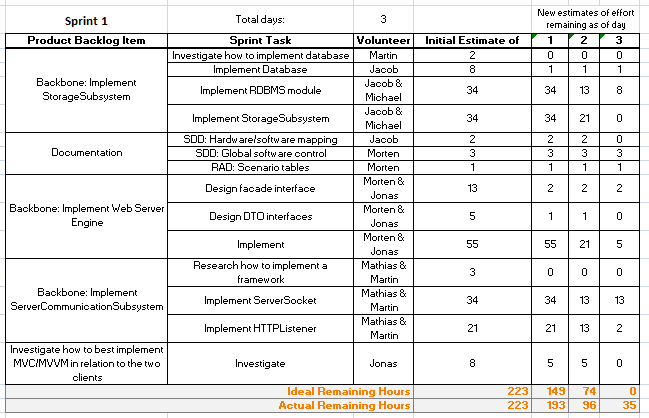
\includegraphics[scale=0.75]{img/backlogSprint1.png}
\caption{Backlog Sprint 1}
\label{fig:Backlog Sprint 1}
\end{figure}

\newpage
\section{Burndown}
Below is the burndown for our first Sprint
\begin{figure}[h]
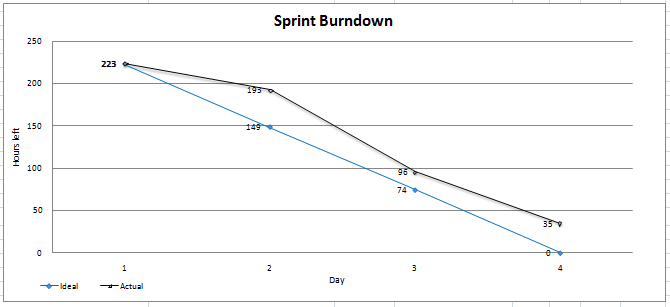
\includegraphics[scale=0.7]{img/burndownSprint1.png}
\caption{Burndown Sprint 1}
\label{fig:Burndown Sprint 1}
\end{figure}


\section{Sprint retrospective}

\begin{center}
\begin{tabular}{|c|c|}
\hline \textbf{What's working well} & \textbf{What could work better} \\ 
\hline Mutual interest in different programming tasks & SCRUM \\ 
Pair Responsibilities(XP) & Pair programming (XP) \\ 
 Time Planning &  \\ 
\hline 
\end{tabular} 
\end{center}



\newpage
\chapter{Sprint 2}
\label{chap:Spring 2}

\section{Backlog}
Below is the backlog for our first sprint
\begin{figure}[h]
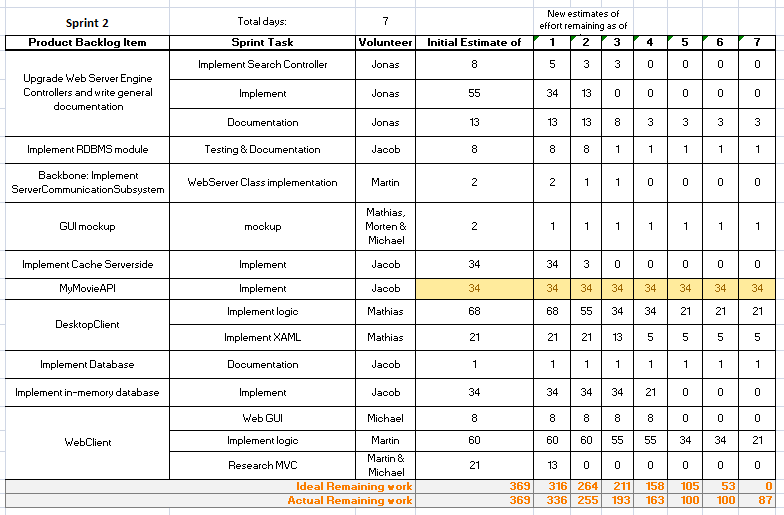
\includegraphics[scale=0.6]{img/backlogSprint2.png}
\caption{Backlog Sprint 2}
\label{fig:Backlog Sprint 2}
\end{figure}

\newpage
\section{Burndown}
Below is the burndown for our first Sprint
\begin{figure}[h]
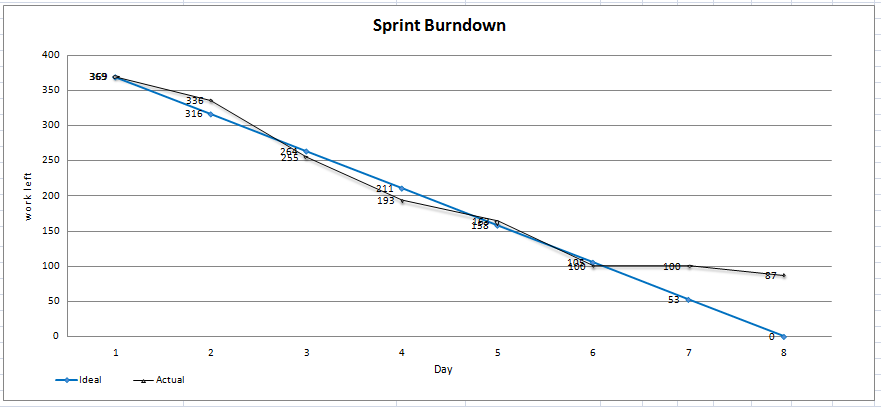
\includegraphics[scale=0.55]{img/burndownSprint2.png}
\caption{Burndown Sprint 2}
\label{fig:Burndown Sprint 2}
\end{figure}


\section{Sprint retrospective}

\begin{center}
\begin{tabular}{|c|c|}
\hline \textbf{What's working well} & \textbf{What could work better} \\ 
\hline No pair programming = more Velocity & Big programming tasks have left some in the cold \\ 
\hline 
\end{tabular} 
\end{center}




\newpage
\chapter{Sprint 3}
\label{chap:Spring 3}

\section{Backlog}


\section{Burndown}


\section{Sprint retrospective}

\begin{center}
\begin{tabular}{|c|c|}
\hline \textbf{What's working well} & \textbf{What could work better} \\ 
\hline Communication & Efficiency \\ 
 Time Planning &  \\ 
 Time Planning &  \\ 
\hline 
\end{tabular} 
\end{center}



\newpage
\chapter{Release Burndown Chart}
\label{chap:Release Burndown Chart}
\begin{center}
%release burndown
\end{center}



\chapter{SCRUM Log}
\label{chap:SCRUM Log}

\section{26. Nov 2013}
This is where we begin our scrum. First we held a start-up meeting where the product owner presented the vision of the system, and afterwards we settled for a definition of done. We also looked at how many hours of available work time we would have for this first sprint. We then moved on the the first part of the meeting for sprint 1. Together we filled the product backlog with scenarios and then estimated the effort. We did the estimation with Fibonacci numbers. After estimating, we, together with the product owner, prioritized the scenarios. Then, moving on to part 2 of the meeting, we choose a bunch from the top with a workload which seemed realistic, and copied them into the sprint backlog. Each scenario we divided into tasks to be done, divided responsibilities and estimated effort. That did it for today. Start up meeting and sprint meetings took just over 4 hours.


\section{27. Nov 2013}
The day started with a stand-up meeting of about 10 minutes. Tasks has been distributed into Trello and assigned accordingly to the sprint start-up meeting. One pig had become ill, and we had several start-up trouble, so we're all looking forward to seeing our sprint burndown chart in the morning.

\section{1. Dec 2013}
Our first sprint is due to end Thursday, and hence almost over. Today people are working from home trying to finish up some tasks for the sprint. We will have to put some unfinished tasks back in the product backlog, but that is not unexpected. There are several things we would like to improve upon to better our scrum, but we will look into those at the sprint retrospective.

\section{10. Dec 2013}
Our second sprint is now over. Our velocity this sprint has been far greater than that in the first, for a couple of reasons: The start-up tasks that we did not calculate for in the first sprint are done, and we have done much less pair programming.

\section{Trello}



\begin{figure}[h]
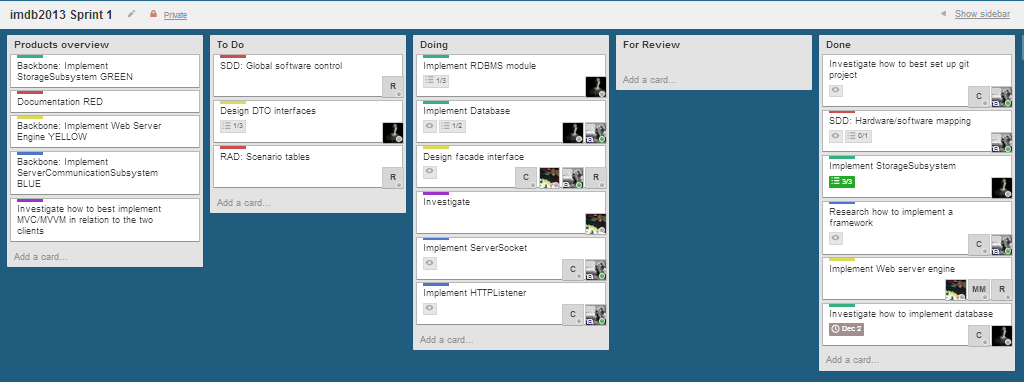
\includegraphics[scale=0.5]{img/trelloSprint1.png}
\caption{Trello Sprint 1}
\label{fig:Trello Sprint 1}
\end{figure}

\begin{figure}[h]
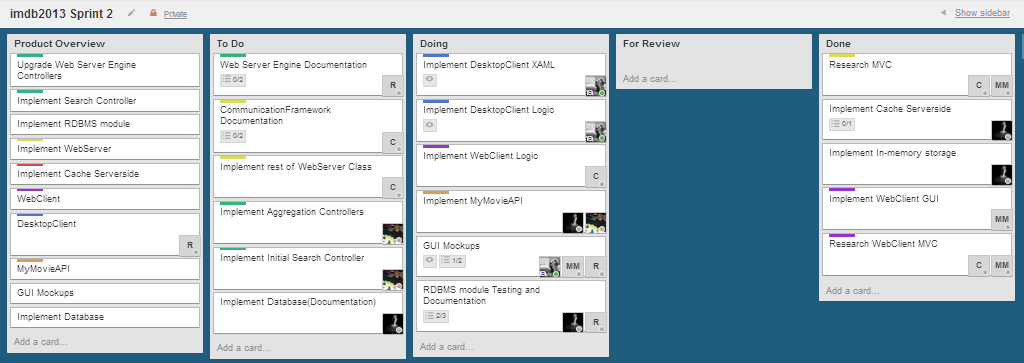
\includegraphics[scale=0.5]{img/trelloSprint2.png}
\caption{Trello Sprint 2}
\label{fig:Trello Sprint 2}
\end{figure}

\begin{figure}[h]
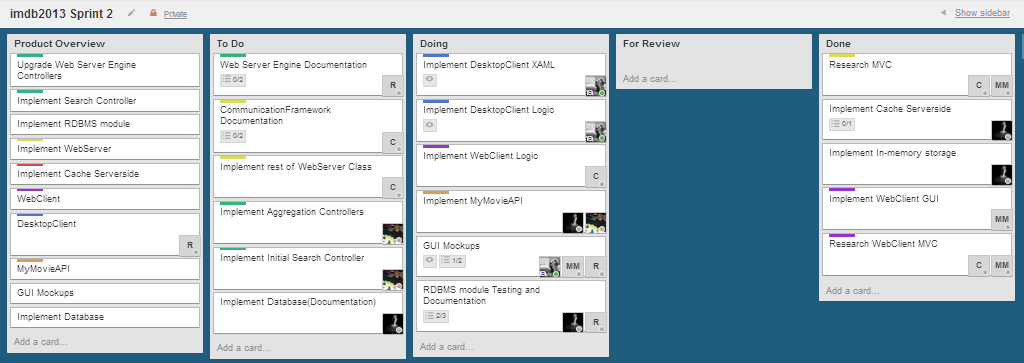
\includegraphics[scale=0.5]{img/trelloSprint2.png}
\caption{Trello Sprint 3}
\label{fig:Trello Sprint 3}
\end{figure}


\end{document}          
